\section{Saules apstarojums}

Lielākā daļa Saules emitētās enerģijas tiek saražota kodolreakcijās fotosfērā. Kopējais saules apstarojums (TSI) ir saņemtā enerģija laika vienībā uz laukuma vienības perpendikulāri starojuma izplatīšanās virzienam 1 AU attālumā integrēta pa visiem viļņu garumiem.\cite{ThermalProcesses} Kopējā saules apstarojuma vērtība mainās laikā, korelē ar Saules plankumu ciklu ~\ref{fig:TSI_misijas}  un norāda uz solārās radiācijas izmaiņām, kas ietekmē solārās enerģijas apjomu uz Zemes atmosfēras augšējiem slāņiem. Papildus ir noderīgi zināt saņemtā starojuma spektrālo sadalījumu -- ~\ref{fig:SSI} redzams, ka aptuveni puse starojuma tiek saņemta 380 -- 780 nm diapazonā, kas padara iespējumu no tā iegūt enerģiju ar saules paneļu paņēmienu.

TSI novērojumi no kosmosa tiek veikti kopš 1978. gada un instrumentu specifikas dēļ iegūtas dažādas absolūtās vērtības ~\ref{fig:TSI_misijas}, tāpēc šī fizikālā lieluma tikai daļēji pārkājušos novērojumu laikrindu apvienošana kompozītā ir gan zinātnisks, gan statistisks izaicinājums un neviens kompozīts (piemēram, PMOD, ACRIM, IRBM) līdz šim nav guvis konsensu solārā apstarojuma pētnieku kopienā.~\ref{fig:TSI_misijas} 

\begin{figure}[h]
    \centering
    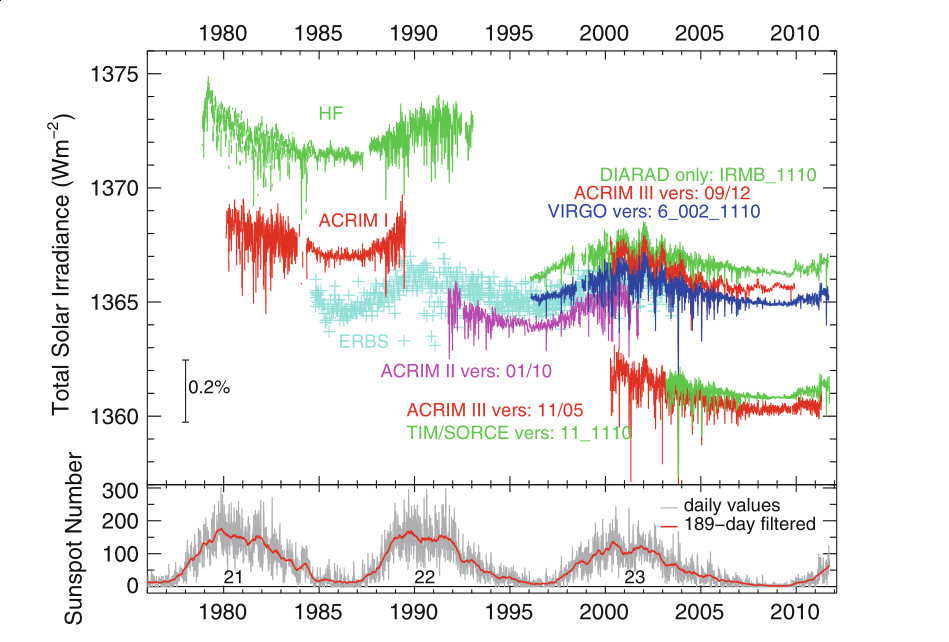
\includegraphics[width=0.6\linewidth]{figures/misc/TSI_misijas.png}
    \caption{Salīdzinājums dienā vidējotiem saules kopējā apstarojuma datiem no dažādām misijām un Saules plankuma skaitlis, lai ilustrētu solārās aktivitātes variabilitāti trīs ciklos. \cite{Frohlich2012}}
    \label{fig:TSI_misijas}
\end{figure}

\begin{table}[h]
    \caption{TSI mērījumu vēsture} % uzrakstīt kādu absolūto TSI izmērīja vai norādīt uz grafiku?
    \begin{center}
    \begin{tabular}{| r | c | l |}
    \hline
    radiometrs & misija & darbības laiks \\ \hline
    Hickey-Frieden & NIMBUS-7 & 1978--1992  \\ \hline
	ACRIM I & Solārā Maksimuma Misija (SMM) & 1980--1989 \\ \hline
	ACRIM  & Zemes Radiācijas Budžeta Satelīts (ERBS) & 1984--2003 \\ \hline
	ACRIM II & Augšējās Atmosfēras Izpētes Satelīts (UARS) & 1991--2001 \\ \hline
	VIRGO & Solārā un Heliosfēras observatorija (SOHO)& 1996--pašlaik \\ \hline
	ACRIM III & ACRIMSAT  & 2000--pašlaik \\ \hline
	TIM & Saules Radiācijas un Klimata Eksperiments (SORCE) & 2003--pašlaik\\ \hline
    \end{tabular}
    \end{center}
    \label{tab:radiometers}
\end{table}

Par labāko saules apstarojuma mērījumu reprezentāciju tiek uzskatīti TIM instrumenta dati mēraparāta uzbūves (atšķirībā no citiem radiometriem TIM precizitātes apertūra atrodas tuvu dobumam un redzeslauku bloķējošā apertūra ir pie instrumenta ieejas) un augstās precizitātes -- nenoteiktība tiek novērtēta esam mazāk nekā $0.014\textrm{Wm}^{-2}\textrm{yr}^{-1}$ un precizitāte ar $0.48\textrm{Wm}^{-2}$ \cite{TSIdata} -- dēļ, tāpēc šajā darbā grafiki balstās uz šiem mērījumiem, pēc kuriem absolūtā kopējā saules apstarojuma vērtība ir $1360.8 \pm 0.5 \textrm{Wm}^{-2}$.\cite{Frohlich2012}

\begin{figure}[h]
    \centering
    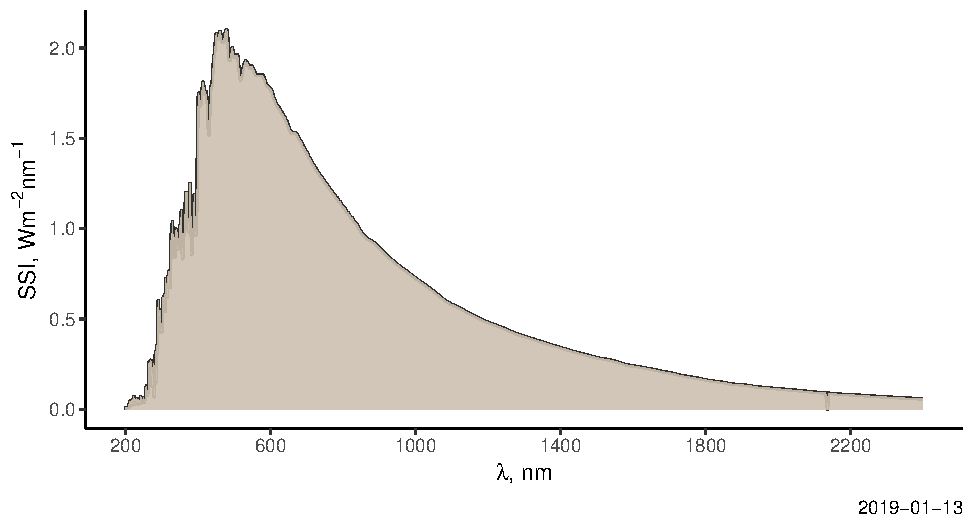
\includegraphics[width=\linewidth]{figures/misc/SSI.pdf}
    \caption{SSI 1AU attālumā (24 h vidējā vērtība) \cite{SSIdata}}
    \label{fig:SSI}
\end{figure}

\begin{figure}[h]
    \centering
    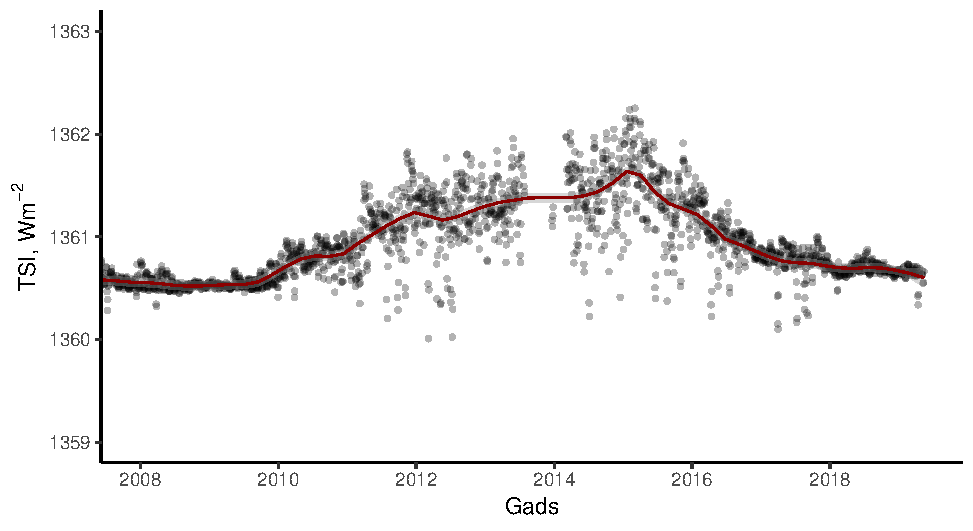
\includegraphics[width=\linewidth]{figures/misc/TSI_8-19.pdf}
    \caption{TSI 24. saules ciklā 1AU attālumā (24 h vidējā vērtība)\cite{TSIdata}}
    \label{fig:TSI1}
\end{figure}

\begin{figure}[h]
    \centering
    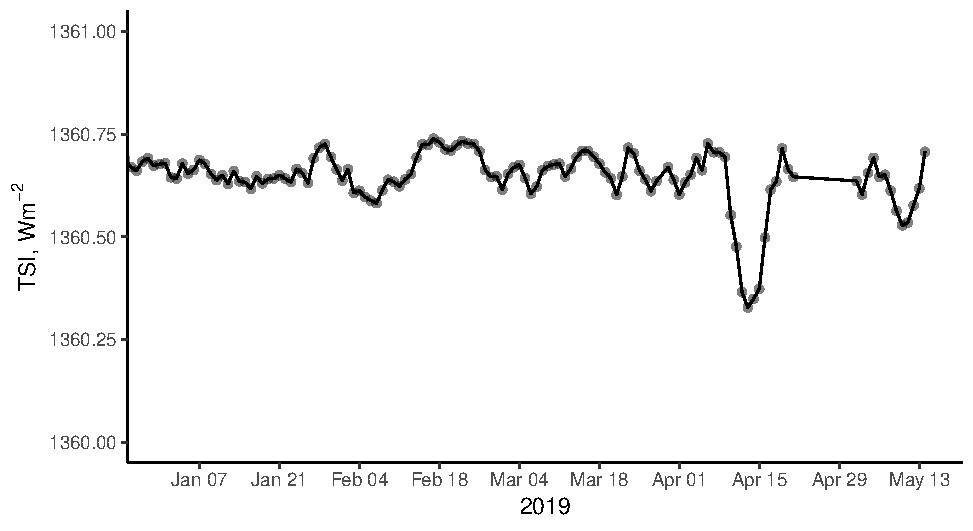
\includegraphics[width=\linewidth]{figures/misc/TSI.pdf}
    \caption{TSI izmaiņas solāro paneļu datu ieguves laikā 1AU attālumā (24 h vidējā vērtība)\cite{TSIdata}}
    \label{fig:TSI2}
\end{figure}

% \begin{figure}[h]
%     \centering
%     \includegraphics[width=\linewidth]{figures/misc/LV_DNI.png}
%     \caption{Tiešais normālais apstarojums \cite{solargis}}
%     \label{fig:lv_DNI}
% \end{figure}
% \begin{figure}[h]
%     \centering
%     \includegraphics[width=\linewidth]{figures/misc/LV_GHI.png}
%     \caption{Globālais horizontālais apstarojums Latvijā \cite{solargis}}
%     \label{fig:lv_GHI}
% \end{figure}
% \begin{figure}[h]
%     \centering
%     \includegraphics[width=\linewidth]{figures/misc/LV_PVOUT.png}
%     \caption{PV potenciālā jauda \cite{solargis}}
%     \label{fig:lv_PVOUT}
% \end{figure}
